\documentclass{article}

\usepackage{graphicx}
\usepackage{tikz}
\usepackage{tikzsymbols}
\usetikzlibrary{calc,patterns,shapes.geometric}
\pagestyle{empty}
\usepackage[margin=0pt]{geometry}
\geometry{papersize={14in,12in}}

\def\centerarc[#1](#2)(#3:#4:#5){\draw[#1] ($(#2)+({#5*cos(#3)},{#5*sin(#3)})$) arc (#3:#4:#5);}

\begin{document}
	\begin{figure}
		\centering
		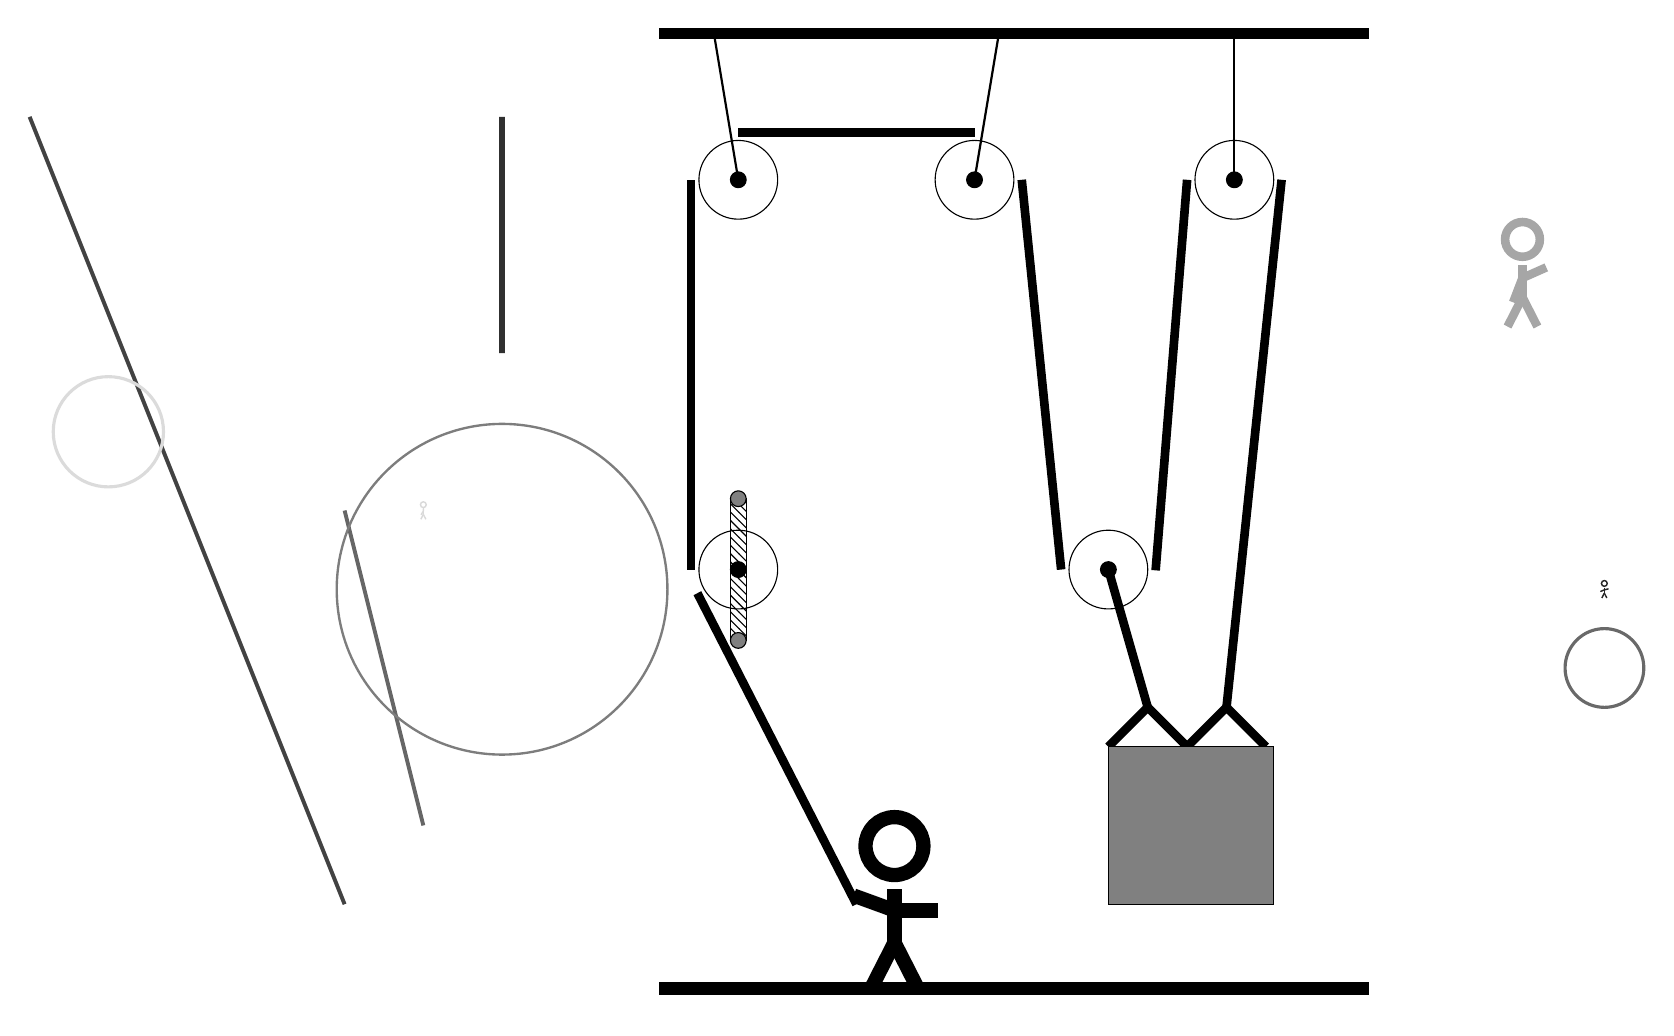
\begin{tikzpicture}
			%%%%% START %%%%%
			
			\draw[fill=black] (-3, 9) rectangle (6, 9.125);
			
			\draw (1, 7.2) circle (0.5);
			\draw[fill=black] (1, 7.2) circle (0.1);
			\draw[thick] (1, 7.2) -- (1.3, 9);
			
			\draw (4.3, 7.2) circle (0.5);
			\draw[fill=black] (4.3, 7.2) circle (0.1);
			\draw[thick] (4.3, 7.2) -- (4.3, 9);
			
			\draw (2.7, 2.25) circle (0.5);
			\draw[fill=black] (2.7, 2.25) circle (0.1);
			
			\draw[line width=1.1mm]  (2.7, 0) -- (3.2, 0.5) -- (3.7, 0) -- (4.2, 0.5) -- (4.7, 0);
			\draw[fill=black!50] (2.7, 0) rectangle (4.8, -2);
			
			\draw (-2, 7.2) circle (0.5);
			\draw[fill=black] (-2, 7.2) circle (0.1);
			\draw[thick] (-2, 7.2) -- (-2.3, 9);
			
			\draw (-2, 2.25) circle (0.5);
			\draw[fill=black] (-2, 2.25) circle (0.1);
			\draw[pattern=north west lines, pattern color=black] (-2.1, 3.15) rectangle (-1.9, 1.35);
			\draw[fill=black!50] (-2, 3.15) circle (0.1);
			\draw[fill=black!50] (-2, 1.35) circle (0.1);
			
			\node[line width=0.7mm, color=black!15] at (-6, 3) {\Strichmaxerl[1][58][87]};
			
			\draw [line width=0.4mm, color=black!59](9, 1) circle (0.5);
			\draw[line width=0.5mm, color=black!60](-6, -1) -- (-7, 3);
			\draw [line width=0.3mm, color=black!51](-5, 2) circle (2.1);
			\node[line width=0.7mm, color=black!35] at (8, 6) {\Strichmaxerl[6][69][24]};
			
			\draw[line width=0.5mm, color=black!74](-7, -2) -- (-11, 8);
			\draw[line width=0.7mm, color=black!81] (-5, 5) rectangle (-5, 8);
			
			\node[line width=0.2mm, color=black!85] at (9, 2) {\Strichmaxerl[1][23][14]};
			\draw [line width=0.4mm, color=black!14](-10, 4) circle (0.7);
			
			\draw[line width=1.1mm](-0.5, -2) -- (-2.5196, 1.95);
			\centerarc[line width=1.1mm](-2, 2.25)(180:210:0.6);
			\draw[line width=1.1mm](-2.6, 2.25) -- (-2.6, 7.2);
			\centerarc[line width=1.1mm](-2, 7.2)(90:180:0.6);
			
			\draw[line width=1.1mm](-2, 7.8) -- (1, 7.8);
			\centerarc[line width=1.1mm](1, 7.2)(0:90:0.6);
			\draw[line width=1.1mm](1.6, 7.2) -- (2.1, 2.25);
			\centerarc[line width=1.1mm](2.7, 2.25)(180:370:0.6);
			\draw[line width=1.1mm] (3.3, 2.24) -- (3.7, 7.2);
			\centerarc[line width=1.1mm](4.3, 7.2)(0:180:0.6);
			\draw[line width=1.1mm](4.2, 0.5) -- (4.9, 7.2);
			\draw[line width=1.1mm] (3.2, 0.5) -- (2.7, 2.25);
			
			\node at (0, -2) {\Strichmaxerl[10][-20][0]};
			
			\draw[fill=black] (-3, -3) rectangle (6, -3.15);
			
			%%%%% END %%%%%
		\end{tikzpicture}
	\end{figure}	
\end{document}